\documentclass{article}
\usepackage[utf8]{inputenc}
\usepackage{amsmath, amssymb, amsthm}
\usepackage{geometry}
\usepackage{enumitem}
\usepackage{CJKutf8}
\usepackage{tikz}
\usetikzlibrary{shapes,arrows,positioning}

\geometry{a4paper, margin=1in}

\title{COMP1046 离散数学复习指南 (Part 1)}
\author{Based on AE1MCS Slides}
\date{2026年1月}

\begin{document}
\begin{CJK*}{UTF8}{gbsn}

\maketitle

\section{命题逻辑 (Propositional Logic)}

\subsection{核心概念}
\begin{itemize}
    \item \textbf{Proposition (命题)}: A declarative statement that is either true or false, but not both.
    \item \textbf{Logical Operators (逻辑运算符)}:
    \begin{itemize}
        \item Negation ($\neg p$)
        \item Conjunction ($p \land q$)
        \item Disjunction ($p \lor q$)
        \item Exclusive OR ($p \oplus q$)
        \item Implication ($p \to q$)
        \item Biconditional ($p \leftrightarrow q$)
    \end{itemize}
    \item \textbf{Definitions}:
    \begin{itemize}
        \item \textbf{Tautology (重言式/永真式)}: Always true.
        \item \textbf{Contradiction (矛盾式/永假式)}: Always false.
        \item \textbf{Contingency (可能式)}: Neither a tautology nor a contradiction.
        \item \textbf{Logical Equivalence (逻辑等价)}: $p \equiv q$ if $p \leftrightarrow q$ is a tautology.
    \end{itemize}
\end{itemize}

\subsection{重要逻辑等价律 (Logical Equivalences)}
熟记以下定律用于化简和证明:
\begin{enumerate}
    \item \textbf{Identity Laws}: $p \land T \equiv p$, $p \lor F \equiv p$
    \item \textbf{Domination Laws}: $p \lor T \equiv T$, $p \land F \equiv F$
    \item \textbf{Idempotent Laws (幂等律)}: $p \lor p \equiv p$, $p \land p \equiv p$
    \item \textbf{Double Negation}: $\neg(\neg p) \equiv p$
    \item \textbf{Commutative Laws (交换律)}: $p \lor q \equiv q \lor p$
    \item \textbf{Associative Laws (结合律)}: $(p \lor q) \lor r \equiv p \lor (q \lor r)$
    \item \textbf{Distributive Laws (分配律)}: $p \lor (q \land r) \equiv (p \lor q) \land (p \lor r)$
    \item \textbf{De Morgan’s Laws (德摩根律)}: $\neg(p \land q) \equiv \neg p \lor \neg q$, $\neg(p \lor q) \equiv \neg p \land \neg q$
    \item \textbf{Absorption Laws (吸收律)}: $p \lor (p \land q) \equiv p$
    \item \textbf{Negation Laws}: $p \lor \neg p \equiv T$
\end{enumerate}

\subsection{蕴含与双蕴含的等价形式}
\begin{itemize}
    \item \textbf{Implication}: $p \to q \equiv \neg p \lor q$
    \item \textbf{Contrapositive (逆否)}: $p \to q \equiv \neg q \to \neg p$
    \item \textbf{Biconditional}: $p \leftrightarrow q \equiv (p \to q) \land (q \to p)$
\end{itemize}

\section{谓词逻辑 (Predicate Logic)}

\subsection{核心概念}
\begin{itemize}
    \item \textbf{Predicates (谓词)}: Statements involving variables (e.g., $P(x)$).
    \item \textbf{Quantifiers (量词)}:
    \begin{itemize}
        \item \textbf{Universal (全称)}: $\forall x P(x)$ ("For all $x$...") $\to$ 常搭配 Implication ($\to$)
        \item \textbf{Existential (存在)}: $\exists x P(x)$ ("There exists an $x$...") $\to$ 常搭配 Conjunction ($\land$)
    \end{itemize}
\end{itemize}

\subsection{量词的否定 (De Morgan’s Laws for Quantifiers)}
\begin{itemize}
    \item $\neg \forall x P(x) \equiv \exists x \neg P(x)$
    \item $\neg \exists x P(x) \equiv \forall x \neg P(x)$
\end{itemize}

\section{推理规则 (Inference Rules)}

\subsection{命题逻辑推理}
\begin{itemize}
    \item \textbf{Modus Ponens}: $(p \land (p \to q)) \to q$
    \item \textbf{Modus Tollens}: $(\neg q \land (p \to q)) \to \neg p$
    \item \textbf{Hypothetical Syllogism (假言三段论)}: $((p \to q) \land (q \to r)) \to (p \to r)$
    \item \textbf{Disjunctive Syllogism (析取三段论)}: $((p \lor q) \land \neg p) \to q$
    \item \textbf{Addition}: $p \to (p \lor q)$
    \item \textbf{Simplification}: $(p \land q) \to p$
    \item \textbf{Resolution}: $((p \lor q) \land (\neg p \lor r)) \to (q \lor r)$
\end{itemize}

\subsection{谓词逻辑推理}
\begin{itemize}
    \item \textbf{Universal Instantiation (全称特指)}: $\forall x P(x) \to P(c)$
    \item \textbf{Universal Generalization (全称推广)}: $P(c) \text{ for arbitrary } c \to \forall x P(x)$
    \item \textbf{Existential Instantiation (存在特指)}: $\exists x P(x) \to P(c)$ (for some element $c$)
    \item \textbf{Existential Generalization (存在推广)}: $P(c) \to \exists x P(x)$
\end{itemize}

\section{证明方法 (Proof Techniques)}

\subsection{常见方法}
\begin{itemize}
    \item \textbf{Direct Proof (直接证明)}: Assume $p$ is true, show $q$ is true.
    \item \textbf{Proof by Contraposition (逆否证明)}: Prove $\neg q \to \neg p$.
    \item \textbf{Proof by Contradiction (反证法)}: Assume $\neg p$, derive a contradiction ($F$).
    \item \textbf{Proof by Cases (分类讨论)}: Prove for exhaustive cases.
    \item \textbf{Proof by Induction (归纳法)}: See Section 4.3 for Weak vs Strong Induction.
\end{itemize}

\subsection{证明格式要求 (Proof Format)}
\begin{itemize}
    \item \textbf{Logic/Set Proofs}: Sequence of equivalences with reasons.
    \item \textbf{Inference Rules}: Steps and reasons clearly listed.
    \item \textbf{Natural Language}: Clear English explanation (Direct, Contraposition, etc.).
\end{itemize}

\subsection{数学归纳法与强归纳法 (Induction)}
\begin{itemize}
    \item \textbf{Weak Induction (第一/普通归纳法)}:
    \begin{itemize}
        \item \textbf{Base Step}: Prove $P(1)$ is true.
        \item \textbf{Inductive Step}: Assume $P(k)$ is true, prove $P(k+1)$ is true.
        \item \textit{Analogy}: Dominoes. If tile $k$ falls, it knocks over $k+1$.
    \end{itemize}
    
    \item \textbf{Strong Induction (强归纳法/第二归纳法)}:
    \begin{itemize}
        \item \textbf{Base Step}: Prove $P(1)$ (sometimes $P(1), \dots, P(b)$ range needed).
        \item \textbf{Inductive Step}: Assume $P(1) \land P(2) \land \dots \land P(k)$ are ALL true, prove $P(k+1)$ is true.
        \item \textit{Key Difference}: You assume the statement holds for \textbf{all} values up to $k$, not just $k$.
    \end{itemize}
    
    \item \textbf{Example of Strong Induction (Prime Factorization)}:
    \newline \textit{Theorem}: Every integer $n \ge 2$ can be written as a product of primes.
    \begin{proof}
        \textbf{Base Case}: For $n=2$, it is a prime number. True.
        \newline \textbf{Inductive Hypothesis (Strong)}: Assume that for all integers $j$ such that $2 \le j \le k$, $j$ can be written as a product of primes.
        \newline \textbf{Inductive Step}: Consider $n = k+1$.
        \begin{itemize}
            \item Case 1: If $k+1$ is prime, then it is a product of (one) prime. True.
            \item Case 2: If $k+1$ is composite, then $k+1 = a \cdot b$ where $2 \le a, b \le k$.
            \item By the Strong Hypothesis, both $a$ and $b$ can be written as products of primes.
            \item Thus, $k+1 = a \cdot b$ is a product of primes.
        \end{itemize}
        Conclusion: By Strong Induction, the statement holds for all $n \ge 2$.
    \end{proof}
\end{itemize}

\section{集合 (Sets)}

\subsection{基础}
\begin{itemize}
    \item \textbf{Notation}: 
    \begin{itemize}
        \item $x \in A$ (Element belongs to set)
        \item $\emptyset$ (Empty Set)
        \item $A \subseteq B$ (Subset)
        \item $|A|$ (Cardinality/Size: number of elements in set A)
    \end{itemize}
    \item \textbf{Power Set (幂集)}: $P(A)$ is the set of all subsets of $A$. 
    \begin{itemize}
        \item If $|A|=n$, then $|P(A)|=2^n$.
        \item \textbf{Important}: The Power Set always includes the Empty Set $\emptyset$ and the set $A$ itself.
        \item Example: If $A=\{1,2\}$, $P(A)=\{\emptyset, \{1\}, \{2\}, \{1,2\}\}$.
    \end{itemize}
    \item \textbf{Cartesian Product}: $A \times B = \{(a, b) \mid a \in A, b \in B\}$.
\end{itemize}

\subsection{集合运算 (Set Operations)}
Union ($A \cup B$), Intersection ($A \cap B$), Difference ($A - B$), Complement ($\overline{A}$).

\subsection{集合恒等式 (Set Identities)}
\begin{itemize}
    \item $A \cap \overline{A} = \emptyset$
    \item $A \cup \overline{A} = U$
    \item De Morgan: $\overline{A \cup B} = \overline{A} \cap \overline{B}$
\end{itemize}

\subsection{例题:利用集合构造器证明第二德·摩根律}
证明 $\overline{A \cap B} = \overline{A} \cup \overline{B}$:
\begin{align*}
\overline{A \cap B} &= \{x \mid x \notin (A \cap B)\} && \text{by defn. of complement} \\
&= \{x \mid \neg (x \in (A \cap B))\} && \text{by defn. of $\notin$} \\
&= \{x \mid \neg (x \in A \land x \in B)\} && \text{by defn. of intersection} \\
&= \{x \mid \neg (x \in A) \lor \neg (x \in B)\} && \text{by De Morgan's law for Logic} \\
&= \{x \mid x \notin A \lor x \notin B\} && \text{by defn. of $\notin$} \\
&= \{x \mid x \in \overline{A} \lor x \in \overline{B}\} && \text{by defn. of complement} \\
&= \{x \mid x \in \overline{A} \cup \overline{B}\} && \text{by defn. of union} \\
&= \overline{A} \cup \overline{B} && \text{by meaning of notation}
\end{align*}

\section{函数 (Functions)}
\begin{itemize}
    \item \textbf{One-to-One (Injective, 单射)}: $f(a) = f(b) \implies a = b$.
    \item \textbf{Onto (Surjective, 满射)}: For every $y$, there exists $x$ such that $f(x) = y$.
    \item \textbf{One-to-one Correspondence (Bijective, 双射)}: Both 1-to-1 and Onto. Invertible.
    \item \textbf{Inverse Function}: $f^{-1}(y) = x$ iff $f(x) = y$.
    \item \textbf{Composition}: $(f \circ g)(x) = f(g(x))$.
\end{itemize}

\section{关系 (Relations)}

\subsection{性质}
\begin{itemize}
    \item \textbf{Reflexive (自反)}: $(a, a) \in R$ for all $a$.
    \newline \textit{Example:} $R=\{(1,1), (2,2), (3,3), (1,2)\}$ on set $\{1,2,3\}$. Everyone must relate to themselves.
    
    \item \textbf{Symmetric (对称)}: $(a, b) \in R \implies (b, a) \in R$.
    \newline \textit{Example:} "is a sibling of". If $A$ is sibling of $B$, then $B$ is sibling of $A$. $R=\{(1,2), (2,1)\}$.

    \item \textbf{Antisymmetric (反对称)}: $(a, b) \in R \land (b, a) \in R \implies a = b$.
    \newline \textit{Example:} "$\le$". If $x \le y$ and $y \le x$, then $x=y$. It implies no "two-way streets" between distinct elements.
    
    \item \textbf{Transitive (传递)}: $(a, b) \in R \land (b, c) \in R \implies (a, c) \in R$.
    \newline \textit{Example:} "$\le$". If $a \le b$ and $b \le c$, then $a \le c$. Also "ancestor of".
\end{itemize}

\subsection{类型}
\begin{itemize}
    \item \textbf{Equivalence Relation (等价关系)}: Reflexive, Symmetric, Transitive.
    \newline \textit{Example:} "=" (Equality), or "congruence modulo $n$" ($a \equiv b \pmod n$).
\end{itemize}

\section{计数 (Counting)}
\begin{itemize}
    \item \textbf{Product Rule}: Multi-step tasks多步任务.
    \item \textbf{Sum Rule}: Mutually exclusive tasks互斥任务.
    \item \textbf{Inclusion-Exclusion (容斥原理)}: $|A \cup B| = |A| + |B| - |A \cap B|$.
    \item \textbf{Division Rule (除法法则)}: If a task results in $n$ outcomes, but $d$ outcomes are considered the same (equivalent), then there are $n/d$ distinct outcomes. (e.g., used to derive $C(n,r)$ from $P(n,r)$).
    
    \vspace{0.5em}
    \textbf{Example (Circular Seating)}: How many ways to seat 4 people (A,B,C,D) around a round table?
    \begin{itemize}
        \item Linear arrangements: $4! = 24$.
        \item Since rotation doesn't change relative positions, each valid seating generates 4 identical rotations.
        \item By Division Rule: $24/4 = 6$.
    \end{itemize}
    \begin{center}
    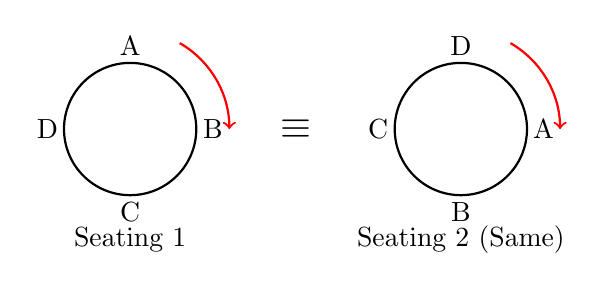
\begin{tikzpicture}[scale=0.7]
      % Circle 1
      \draw[thick] (0,0) circle (1.2cm);
      \node at (90:1.5) {A}; \node at (0:1.5) {B}; \node at (270:1.5) {C}; \node at (180:1.5) {D};
      \draw[->, thick, red] (60:1.8) arc (60:0:1.8);
      \node at (0, -2) {Seating 1};
      
      % Symbol
      \node at (3,0) {\Large $\equiv$};
      
      % Circle 2
      \begin{scope}[xshift=6cm]
      \draw[thick] (0,0) circle (1.2cm);
      \node at (90:1.5) {D}; \node at (0:1.5) {A}; \node at (270:1.5) {B}; \node at (180:1.5) {C};
      \draw[->, thick, red] (60:1.8) arc (60:0:1.8);
      \node at (0, -2) {Seating 2 (Same)};
      \end{scope}
    \end{tikzpicture}
    \end{center}

    \item \textbf{Pigeonhole Principle (鸽巢原理)}: If $k+1$ objects are placed in $k$ boxes, at least one box contains $\ge 2$ objects.
    \item \textbf{Permutations (排列)}: $P(n, r) = \frac{n!}{(n-r)!}$. Order matters.
    \newline \textit{Note:} Often denoted as $A_n^r$. Calculation: $n \times (n-1) \times \dots \times (n-r+1)$.
    \item \textbf{Combinations (组合)}: $C(n, r) = \binom{n}{r} = \frac{P(n,r)}{r!} = \frac{n!}{r!(n-r)!}$. Order doesn't matter.
    \newline \textit{Shortcut:} $\binom{n}{r} = \binom{n}{n-r}$.
\end{itemize}

\section{概率 (Probability)}
\begin{itemize}
    \item \textbf{Probability of Event}: $P(E) = \frac{|E|}{|S|}$ (for equally likely outcomes).
    \item \textbf{Conditional Probability}: $P(E|F) = \frac{P(E \cap F)}{P(F)}$.
    \item \textbf{Bayes’ Theorem}: $P(F|E) = \frac{P(E|F)P(F)}{P(E|F)P(F) + P(E|\neg F)P(\neg F)}$.
    \item \textbf{Expected Value (期望)}: $E(X) = \sum x p(x)$.
    \item \textbf{Variance (方差)}: $V(X) = E((X - E(X))^2) = E(X^2) - E(X)^2$.
\end{itemize}

\section*{考试建议 (Suggestions)}
\begin{itemize}
    \item \textbf{Be well-prepared!} 理解概念和定义。
    \item \textbf{Practice}: 尝试解决教科书中的问题。
    \item \textbf{Express clearly}: 用简单的英语表达,言简意赅。
    \item \textbf{Proof Format}: 注意证明题的格式要求(如列出使用的逻辑律名称)。
\end{itemize}

\end{CJK*}
\end{document}
